\section{Recursive Systematic Convolutional Codes:Review}
\label{sec3}
A rate $R=k/n$ recursive systematic convolutional (RSC) code receives an input of $k$ bits and outputs $n$ bits at each time instance. The output bits are generated using feedback and feedforward connections of a shift register determined by generator functions. The generator function for the RSC code may be written in polynomial notation as $\Big[1 ~\frac{f(x)}{g(x)}\Big]$, where $f(x)$ and $g(x)$ represent the feedforward and feedback connections of the shift register respectively. Also, $1$ represents the systematic (input) bits  that make up the output.

We only focus on the parity part of the RSC code specified by the generator function $\frac{f(x)}{g(x)}$

%An $(n,k)$ RSC code is a convolutional code generated using feedback shift registers. They are known as systematic codes because the input bits are a part of the codeword. At each time instant, it receives an input of $k$ bits and outputs $n$ bits.
%The output bits are determined by the generator function, which may be written in polynomial notation as  $\Big[1 ~\frac{f(x)}{g(x)}\Big]$. Given the systematic nature of the RSC code, we only focus on the parity part of the RSC code and write the generator function simply as $\Big[\frac{f(x)}{g(x)}\Big]$ where $f(x)$ and $g(x)$ represent the feedforward and feedback connections of the RSC encoder.  

Then, the impulse response caused by the feedback connection of the RSC encoder is easily calculated as 
$$\phi_g(x)=g^{-1}(x)$$
and its equivalent vector representation takes the form, 
$$\dot{\bphi_g}$$
where $\bphi_g$ is known as the cycle of the RSC code and $\tau$ is the cycle length. 

The impulse response of the RSC code is calculated as $$\phi(x)=f(x)\phi_{g}(x)$$ 
By careful observation, we can choose two integer values $h ~ \text{and}~ r$ such that we can write the equivalent vector representation as $$\bphi=\bphi_h\dot{\bphi_r}$$

The minimum distance ($d_{\text{min}}$) of the RSC code determines its error-correcting capability. With the aid of the distance spectrum, it is possible to determine $d_{\text{min}}$ as well as its multiplicity. The most common way to find the distance spectrum is via the transfer function of the RSC code. The transfer function enumerates all the paths that diverge from and then return to the initial state \cite{ref3}, \textit{i.e.} the RTZ inputs. In other words, the distance spectrum provides information about the number of codewords of weight $d$ generated by an RTZ input of weight $w$. Combined with the knowledge that all RTZ inputs are divisible by $g(x)$ \cite{ref6}, we introduce a novel method for determining the pattern of the input bits which cause low-weight codewords of any RSC code in the next section. We refer to this method as the  \textit{codeword pattern distance spectrum}. This version of the distance spectrum is a better tool for interleaver design compared to the regular distance spectrum.

\begin{figure}[h]
\centering
		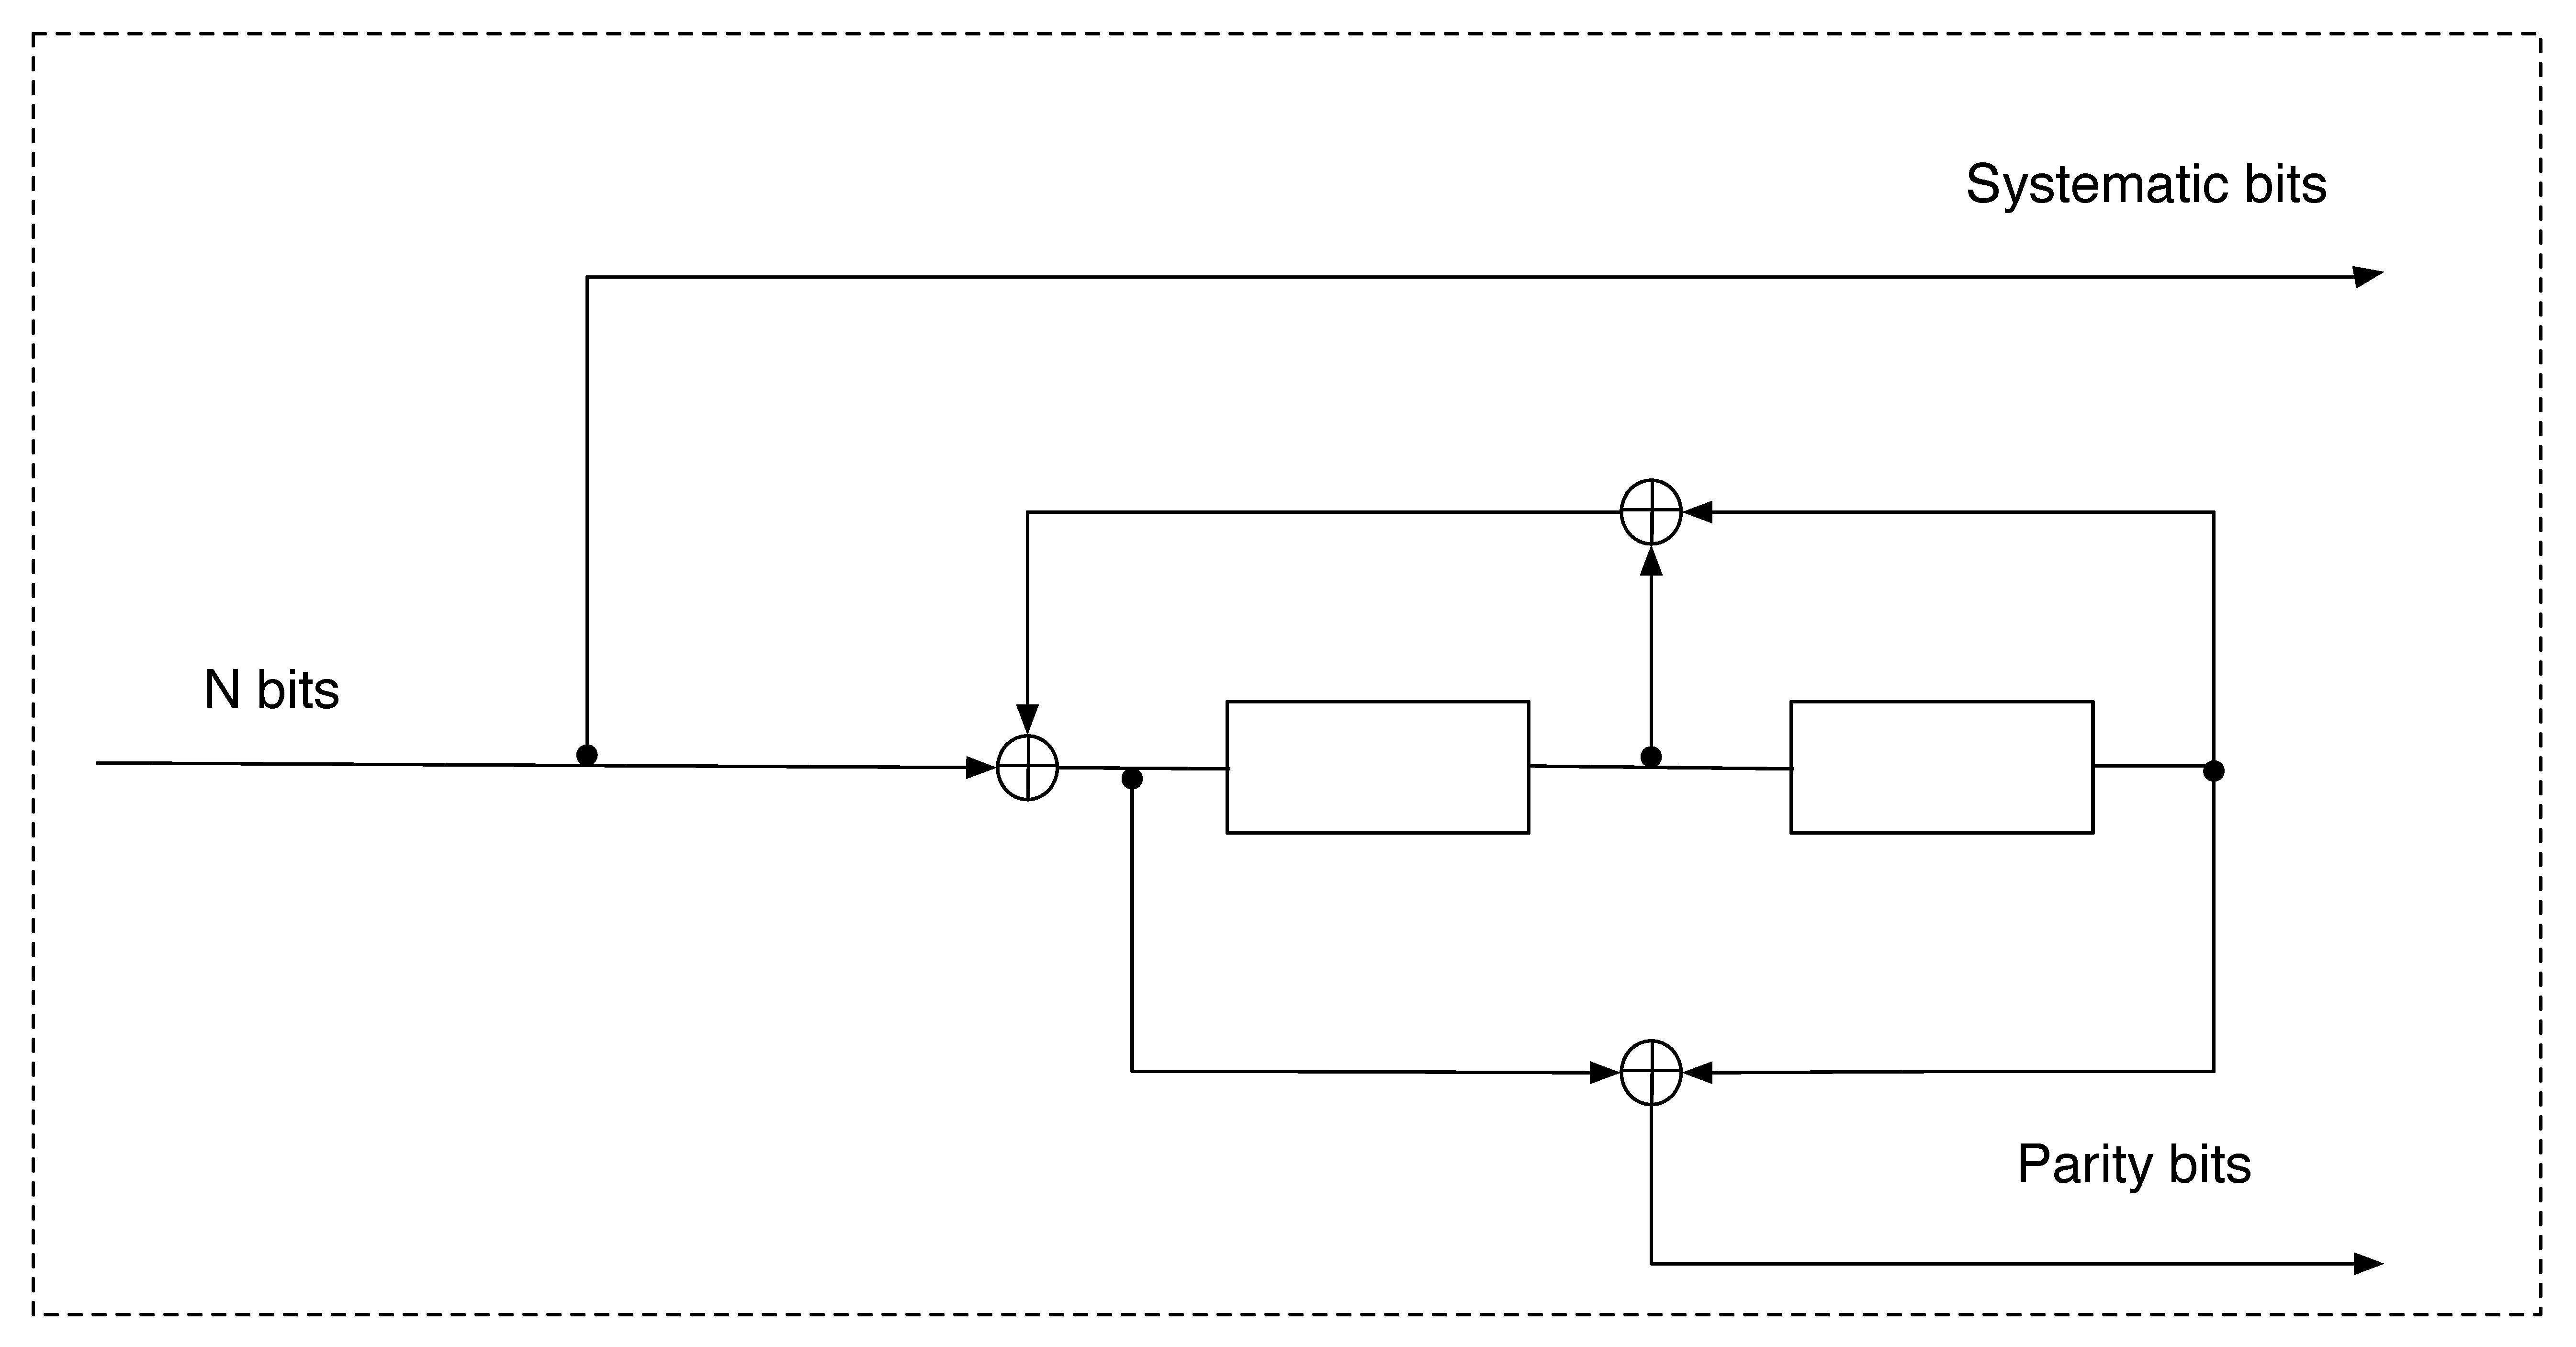
\includegraphics[width=0.45\textwidth]{./PaperSources/RSCExample3.pdf}
		\caption{$[\frac{1+x^2}{1+x+x^2}]$  RSC Encoder}
		\label{fig1}
		\end{figure}

\begin{example}		
An RSC encoder is shown in Figure \ref{fig1} with $k=1$ and $n=2$. Its parity generator\newline function is given by $[\frac{1+x^2}{1+x+x^2}]$, which may be written as $5/7$ in octal form, where $5 ~ \text{and} ~ 7$ correspond to the numerator and denominator of the generator function, respectively. 
 For this RSC code, the cycle is $\bphi_g=\bphi_6 $ with a cycle length $\tau =3$. While $\bphi=(1~1~1~ 0~ 1~ 1~ 0~ 1~ 1~ 0~\cdots)$, which may be written in terms of the elements of GF(8) as $\bphi_7~\dot{\bphi_3}$ represents the impulse response. 
 \end{example}
  Moving forward all other examples and discussions relating to RSC codes will be done using the $5/7$ RSC code unless otherwise stated.

 %The knowledge of $\textbf{p}$ and $\tau$ will be used in deriving the method for determing which input messages generate low-weight parity bits. 